\chapter{PROJECT DESIGN AND IMPLEMENTATION}
\label{ch:Project Design and Implementation}
This chapter presents the design and implementation of the autonomous parcel delivery navigation system. It covers the development approach, performance metrics, software architecture, algorithm design, simulation setup, and prototype demonstration. The chapter explains the step-by-step development process and testing methods used to ensure the system operates reliably and efficiently in complex indoor environments.
\section{Proposed Design Methodology}

The parcel delivery system design method combines a web management integration system, the ROS2 (Robot Operating System 2) navigation system, along with a web-based simulation and visualization of autonomous navigation and a web-based automation system. The system integrates management, real-time monitoring of delivery robots, map management, and the ability to visualize robot operations.

Figure~\ref{overall}At the top are the live telemetry and task options along with the maps and logs which are all accessible via the web interface. The web interface is connected to the backend in Flask. From there it's application logic, REST APIs and database, as well as interface between the web and ROS2. The communication layer robs towards the coordination for the navigation stack, the Gazebo simulation, RViz, and the TurtleBot3. The components of the navigation stack are the Improved A* with Particle Swarm Optimization (PSO) for path smoothing, and Model Predictive Controller (MPC) for path and tracking. The simulation for the navigation of the robot is provided by Gazebo, while the visualizations by RViz for the maps, planned paths, and the robot's telemetry are also real time.
The project is outlined into six development stages:

\begin{figure}[H]
	\centering
	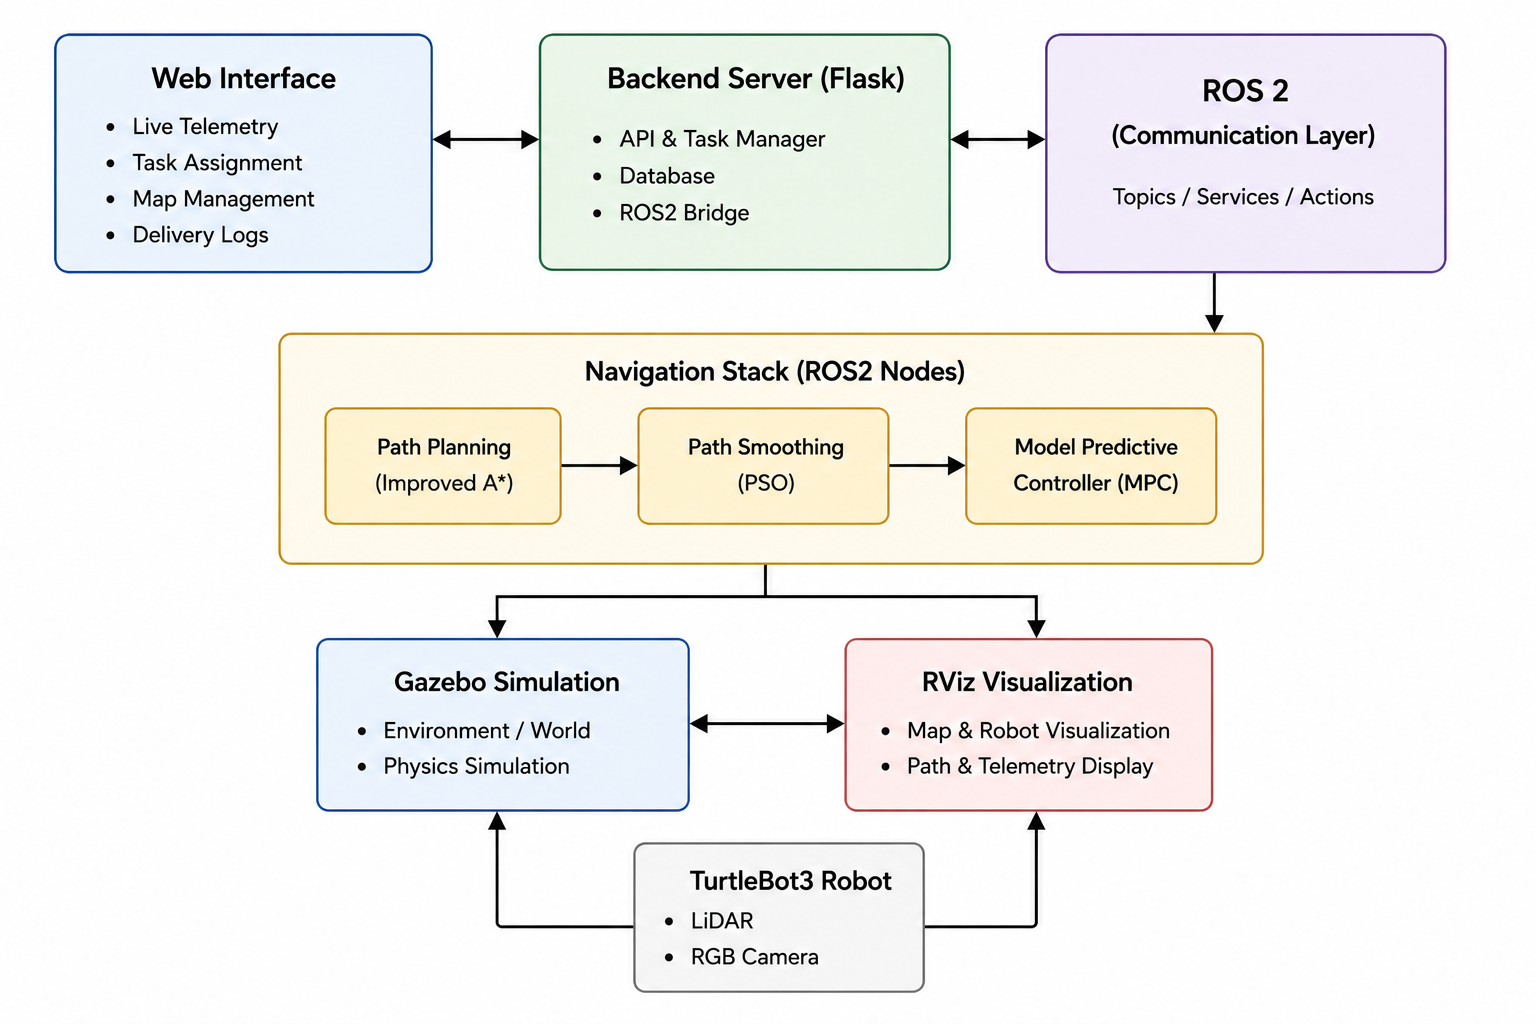
\includegraphics[width=1\textwidth]{overall architecture.png}
	\caption{Overall Architecture of the Proposed Autonomous Parcel Delivery System}
	\label{overall}
\end{figure}

\subsection*{Phase 1: Navigation Algorithm Development}

To create collision-free global paths in the simulation, the Improved A* path planning algorithm was applied. Then, Particle Swarm Optimization (PSO) path smoothing was used to create paths that were shorter, smoother, and more practical for autonomous navigation.
\subsection*{Phase 2: Web-Based Management Platform Development}

A Flask-based application based on Flask for users to easily assign delivery tasks, view real time delivery robot telemetry, manage occupancy maps, and view delivery logs. The interface is the main point of user interaction with the autonomous delivery system.

\subsection*{Phase 3: Backend and ROS2 Integration}

To create smooth connection between the online platform and the robotic system, the backend server was linked with ROS2. While robot status and telemetry data are continuously sent back to the web interface, user commands, delivery objectives, and map management requests are routed to ROS2.

\subsection*{Phase 4: Model Predictive Control Implementation}

To precisely track the optimum navigation path produced by the planning module, a Model Predictive Controller (MPC) was put into place. Smooth and stable autonomous mobility is achieved by the controller's computation of suitable velocity commands while meeting the robot's kinematic limitations.

\subsection*{Phase 5: Simulation and Visualization Integration}
Gazebo and RViz were integrated with the entire navigation stack. While RViz delivers real-time viewing of occupancy maps, robot position, planned trajectories, and navigation status during autonomous deliveries, Gazebo offers a realistic simulation environment for assessing robot performance.


\subsection*{Phase 6: System Deployment and Validation}

Ubuntu 22.04, ROS2, Gazebo, and the TurtleBot3 robot model with LiDAR and RGB camera sensors were used to implement the whole autonomous package delivery system. To verify task execution, autonomous navigation, path tracking, and communication between the web interface and the robotic platform, end-to-end testing was carried out.



\subsection{Overall System Architecture}

A web-based user interface, backend processing, robotic middleware, simulation environment, and the autonomous mobile robot are all integrated into the modular architecture of the suggested autonomous parcel delivery system. Figure~\ref{fig:system_architecture} shows the general workflow of the suggested system, starting with the assignment of tasks to users and concluding with the effective completion of deliveries.

In order to assign delivery jobs and track the robot's real-time telemetry during the delivery process, the user engages with the Web Interface at the highest level. The Backend, which handles user requests and acts as a communication link between the web application and the robotic system, is communicated with using the web interface.

The ROS2 Communication Layer, which serves as the middleware in charge of information exchange between the robot and the software components, is integrated with the backend. In the Gazebo Simulation environment, where the TurtleBot3 robot completes autonomous parcel delivery tasks under realistic simulation conditions, the navigation system is assessed.

The TurtleBot3 Robot has an RGB camera for visual perception and a LiDAR sensor for obstacle recognition and localization. The robot automatically follows the designated delivery path and arrives at the designated destination using the navigation algorithms built into the ROS2 framework, all the while continuously sending telemetry updates to the web interface.

User interaction, backend services, robotic middleware, simulation, and robot operation are all clearly separated thanks to this modular architecture. Scalability, maintainability, and future integration with actual robot hardware are all enhanced by such a design.


\begin{figure}[H]
	\centering
	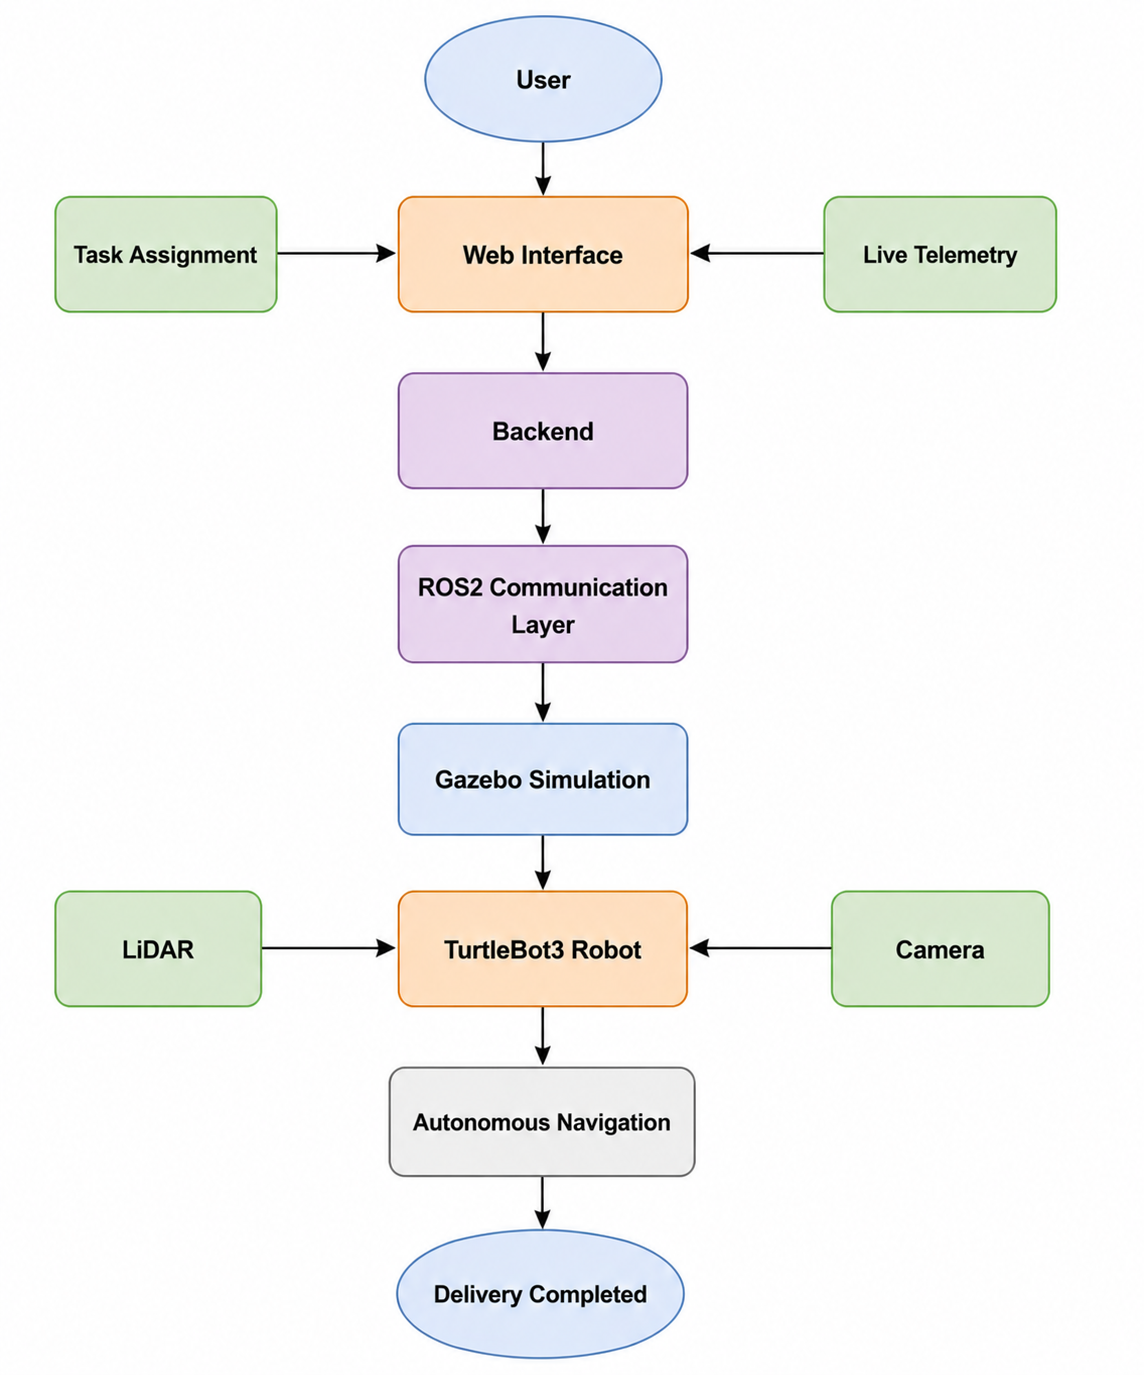
\includegraphics[width=0.8\textwidth]{overflow.png}
	\caption{Overall System Architecture of the Proposed Autonomous Parcel Delivery System}
	\label{fig:system_architecture}
\end{figure}
\section{Implementation Procedure}
\section{Phase 1: Global Path Planning}
\label{sec:phase1_astar}

The global route planning module, which is the first part of the six-phase development approach, is fully designed and implemented in this section. The global planner in charge of creating collision-free pathways throughout the occupancy grid representation of the workspace was chosen to be the Improved A* (IA*) algorithm.


\subsection{Why A*}
\label{subsec:why_astar}

For global path planning, A* algorithm was implemented for its heuristic search efficiency and optimality guarantees. In contrast to ignorant search algorithms like Dijkstra's algorithm, A* employs a heuristic function to steer the search in the direction of the objective. When an admissible heuristic is employed, this drastically reduces the number of nodes examined while still ensuring the shortest path.

The following are the main justifications for using A* as the global planner:


\begin{itemize}[noitemsep]
\item \textbf{Optimality:} When employing an acceptable heuristic (Euclidean distance), A* ensures the shortest collision-free path between the start and target nodes.
\item \textbf{Completeness:} If there is a solution in the occupancy grid, the algorithm will discover it.
\item \textbf{Heuristic-guided efficiency:} Compared to exhaustive search techniques, the Euclidean distance heuristic reduces computer overhead by focusing the search on the objective.
\item \textbf{Grid compatibility:} A* is readily suitable to the workspace representation used in this project because it functions natively on discretized occupancy grid maps.
\item \textbf{Deterministic behavior:} A* simplifies testing and validation by generating repeated, consistent paths for a given map and start/goal setup.

\end{itemize}

In order to overcome the discontinuities and abrupt turns that come with grid-based planning, A* was used as the main global path planner. Its output was then improved through path trimming and PSO-based smoothing (Phase 2).



\subsection{A* Implementation}
\label{subsec:astar_implementation}

A grid-based workspace representation is used in the Python implementation of the A* path planning algorithm. A consistent grid with adjustable resolution is created by discretizing the environment. Based on the locations of obstacles, each grid cell is categorized as either occupied or free area. The technique employs a priority queue to choose nodes with the lowest cost function while maintaining open and closed sets for node exploration:


\begin{equation}
	f(n) = g(n) + h(n)
	\label{eq:astar_cost_impl}
\end{equation}

where $g(n)$ is the actual cost from the start node to the current node, and $h(n)$ is the heuristic estimate from the current node to the goal node.

\subsubsection*{Path Pruning}

Path pruning is employed to remove redundant waypoints produced by A* algorithm. This is done by the pruning algorithm. It goes from one waypoint to the next deleting intermediate spots that do not improve the path quality. A line-of-sight check is performed to ensure a collision-free connection between non-consecutive waypoints.


\subsubsection*{Backend Implementation File}

The backend implementation of the A* algorithm is in \texttt{astar\_modified.py}, which contains the modified A* path planning algorithm tailored to the specific constraints of the project (dynamic safety margin, adaptive grid resolution and 8-directional motion model, see Section ~\ref{subsec:astar_parameters}).


\subsection{Mathematical Model}
\label{subsec:astar_math_model}

The path planning process is modeled as a graph search problem where the environment is divided into a discrete grid. The A* algorithm evaluates nodes using the cost function:

\begin{equation}
	f(n) = g(n) + h(n)
	\label{eq:astar_cost}
\end{equation}

where:
\begin{itemize}[noitemsep]
	\item $g(n)$ = actual cost from start node to current node
	\item $h(n)$ = heuristic estimate from current node to goal node
\end{itemize}

The Euclidean distance heuristic is used, as it is admissible (never overestimates the true cost) and thus preserves the optimality of the A* search:

\begin{equation}
	h(n) = \sqrt{(x_{goal} - x_{current})^2 + (y_{goal} - y_{current})^2}
	\label{eq:euclidean_heuristic_p1}
\end{equation}

Dynamic programming techniques are used to store optimal sub-path solutions, improving computational efficiency through memoization.

\subsection{Parameters}
\label{subsec:astar_parameters}

The A* path planning algorithm is configured with the following adaptive parameters:

\begin{description}[leftmargin=0cm, labelindent=0cm, itemsep=0.3em, font=\normalfont]
	\item[Grid Resolution:] The grid resolution adapts to workspace dimensions to balance computational efficiency and path accuracy:
	\begin{equation}
		\text{resolution} = \min(\text{width}, \text{height}) \times 0.01
	\end{equation}
	
	\item[Safety Margin:] A dynamic safety margin is applied around obstacles to prevent collisions:
	\begin{equation}
		\text{safety\_margin} = \text{resolution} \times 0.2 \text{ meters}
	\end{equation}
	
	\item[Motion Model:] The robot uses an 8-directional motion model with diagonal movement cost of $\sqrt{2} \times \text{resolution}$.
	
	\item[Grid Indexing Formula:] Each cell is assigned a unique index for efficient lookup:
	\begin{equation}
		\text{index} = y_{\text{index}} \times x_{\text{width}} + x_{\text{index}}
	\end{equation}
	
	\item[Heuristic Function:] Euclidean distance is used as the admissible heuristic for optimal pathfinding.
\end{description}

Table~\ref{tab:astar_parameters} summarizes the A* configuration parameters.

\begin{table}[H]
	\centering
	\caption{A* Algorithm Parameters and Configuration}
	\label{tab:astar_parameters}
	\begin{tabular}{|p{4cm}|p{3cm}|p{6.5cm}|}
		\hline
		\textbf{Parameter} & \textbf{Type} & \textbf{Value/Formula} \\
		\hline
		Grid Resolution & Adaptive & $\min(\text{width}, \text{height}) \times 0.01$ \\
		\hline
		Safety Margin & Dynamic & $\text{resolution} \times 0.2$ m \\
		\hline
		Motion Model & 8-directional & Diagonal cost $= \sqrt{2} \times \text{resolution}$ \\
		\hline
		Heuristic Function & Euclidean & $\sqrt{(x_g - x_c)^2 + (y_g - y_c)^2}$ \\
		\hline
		Grid Indexing & Formula & $y_{index} \times x_{width} + x_{index}$ \\
		\hline
	\end{tabular}
\end{table}


\section{Phase 2: Path Optimization}
\label{sec:phase2_optimization}

Following global path generation by the A* planner (Section~\ref{sec:phase1_astar}), the raw path is refined through a two-stage optimization pipeline: path pruning to eliminate redundant waypoints, followed by Particle Swarm Optimization (PSO)-based smoothing to produce a continuous, kinematically feasible trajectory suitable for differential-drive robot motion.

\subsection{Path Pruning}
\label{subsec:path_pruning}

On an 8-directional grid, the raw path produced by A* usually has a lot of closely spaced, collinear, or near-collinear waypoints that are not necessary for smooth trajectory execution and are computationally costly to monitor. Prior to PSO smoothing, path pruning is used as the initial optimization step to minimize this redundancy.

The pruning method eliminates intermediate points that don't improve path quality by iterating through successive waypoints. To ensure collision-free connection, a line-of-sight check is carried out between non-consecutive waypoints. All intermediate waypoints between two non-adjacent waypoints are eliminated if a straight line between them does not cross any obstacles (within the safety margin).
By eliminating needless zigzag segments added by the grid-based search, this step considerably lowers waypoint density while also somewhat reducing the overall path length.


\subsection{Results}
\label{subsec:astar_results}

The A* global planner was tested in two simulated indoor test scenarios of different complexity and scale with the path planning performance indicators (path length, waypoint density, and computing efficiency). The pruned path (after removing redundant waypoints, see Section~\ref{subsec:astar_implementation}) and the raw output of the A* were both recorded for comparison.

\subsubsection*{Scenario 1: M4 Map (100 $\times$ 100 m)}

\textbf{Start:} $(35.0, 95.0)$ \quad \textbf{Goal:} $(50.0, 8.0)$ \\
\textbf{Grid Resolution:} 2.0 m \quad \textbf{Safety Margin (Inflation):} 3.0 m

\begin{table}[H]
	\centering
	\caption{A* Path Planning Results -- Scenario 1 (M4 Map)}
	\label{tab:astar_results_scenario1}
	\begin{tabular}{|p{4.5cm}|p{4cm}|p{4cm}|}
		\hline
		\textbf{Metric} & \textbf{Raw A* Path} & \textbf{Pruned A* Path} \\
		\hline
		Path Length & 100.62 meters & 96.13 meters \\
		\hline
		Waypoint Count & 47 waypoints & 6 waypoints \\
		\hline
		\multicolumn{3}{|c|}{Computation Time: IA* $\approx$ 0.1346 s \quad A* $\approx$ 0.1410 s} \\
		\hline
	\end{tabular}
\end{table}

\subsubsection*{Scenario 2: Mobile Robot Workspace (160 $\times$ 160 m)}

\textbf{Start:} $(5.0, 155.0)$ \quad \textbf{Goal:} $(155.0, 5.0)$ \\
\textbf{Grid Resolution:} 3.0 m \quad \textbf{Safety Margin (Inflation):} 3.0 m

\begin{table}[H]
	\centering
	\caption{A* Path Planning Results -- Scenario 2 (Mobile Robot Workspace)}
	\label{tab:astar_results_scenario2}
	\begin{tabular}{|p{4.5cm}|p{4cm}|p{4cm}|}
		\hline
		\textbf{Metric} & \textbf{Raw A* Path} & \textbf{Pruned A* Path} \\
		\hline
		Path Length & 244.99 meters & 233.87 meters \\
		\hline
		Waypoint Count & 69 waypoints & 5 waypoints \\
		\hline
		\multicolumn{3}{|c|}{Computation Time: IA* $\approx$ 0.4181 s \quad A* $\approx$ 0.4135 s} \\
		\hline
	\end{tabular}
\end{table}

\subsubsection*{Key Observations}

\begin{itemize}[noitemsep]
\item \textbf{Identical paths between planners:} In all cases, the Improved A* (IA*) planner and the conventional A* planner produce similar paths (with the same length and number of waypoints) because obstacles prevent a straight line from start to goal, and both planners are forced to rely on the entire grid search. The difference in computation time between the two planners is minimal.
\item \textbf{Effectiveness of pruning:} The path pruning step reduces significantly the waypoint density and the total path length by eliminating useless zigzag segments generated by the 8-directional grid search:

\begin{itemize}[noitemsep]
	\item In Scenario~1, waypoint pruning reduced the number of waypoints from 47 to 6, representing an 87.2\% reduction, while shortening the path length by 4.49~m, from 100.62~m to 96.13~m.
	
	\item In Scenario~2, waypoint pruning reduced the number of waypoints from 69 to 5, corresponding to a 92.8\% reduction, and decreased the path length by 11.12~m, from 244.99~m to 233.87~m.
\end{itemize}	
\end{itemize}

\subsection{Particle Swarm Optimization (PSO)}
\label{subsec:pso_overview}
Pruning will eliminate useless waypoints, but the resulting path may contain sharp turns and discontinuities of the curvature that are incompatible with the kinematic specifications of a differential-drive robot. The path is further smoothed by the aid of Particle Swarm Optimization (PSO) for improving the trajectory feasibility and reducing the sharp curves.

Each swarm particle is a candidate smoothed path and the position variables of each particle are the coordinates of the way points between the smoothed path particles. Each iteration, the swarm updates the position of each particle according to the velocity equations, all the while keeping an eye on a cost function that combines path length, smoothness and obstacle proximity. The swarm moves towards a path which is balancing these conflicting goals.
\subsection{Cost Function}
\label{subsec:pso_cost_function}

The PSO smoothing process optimizes a multi-objective cost function that is a combination of three weighted components:

\begin{equation}
	J = w_1 \cdot L + w_2 \cdot C + w_3 \cdot P
	\label{eq:pso_cost_p2}
\end{equation}

where:
\begin{itemize}[noitemsep]
	\item $L$ = total path length
	\item $C$ = curvature or smoothness factor
	\item $P$ = obstacle penalty function
	\item $w_1, w_2, w_3$ = weighting coefficients
\end{itemize}

Smaller values of $J$ correspond to shorter, smoother and safer routes. The penalty term $P$ for obstacle grows rapidly when the candidate path is close to or crosses an obstacle boundary, discouraging the swarm from converging to infeasible trajectories.

\subsection{Equations}
\label{subsec:pso_equations}

Particle position and velocity updates follow the standard PSO formulation:

\begin{align}
	v_i(t+1) &= w \cdot v_i(t) + c_1 \cdot r_1 \cdot (p_{best,i} - x_i(t)) + c_2 \cdot r_2 \cdot (g_{best} - x_i(t)) \label{eq:pso_velocity_p2} \\
	x_i(t+1) &= x_i(t) + v_i(t+1) \label{eq:pso_position_p2}
\end{align}

where:
\begin{itemize}[noitemsep]
	\item $w$ = inertia weight, controlling the influence of a particle's previous velocity
	\item $c_1, c_2$ = cognitive and social coefficients, weighting a particle's attraction to its own best-known position and the swarm's best-known position respectively
	\item $r_1, r_2$ = random values in $[0,1]$, introducing stochastic variation into the search
	\item $p_{best,i}$ = personal best position found by particle $i$
	\item $g_{best}$ = global best position found by the entire swarm
\end{itemize}

At each iteration, every particle's cost $J$ (Equation~\ref{eq:pso_cost_p2}) is evaluated, and $p_{best,i}$ and $g_{best}$ are updated whenever a particle discovers a lower-cost path. This process repeats until a maximum number of iterations is reached or convergence criteria are satisfied.

\subsection{Parameters}
\label{subsec:pso_parameters}

Particle Swarm Optimization is configured with the following parameters to balance exploration and exploitation:

\begin{table}[H]
	\centering
	\caption{PSO Algorithm Parameters}
	\label{tab:pso_parameters_p2}
	\begin{tabular}{|p{6cm}|p{2cm}|p{2cm}|}
		\hline
		\textbf{Parameter} & \textbf{Symbol} & \textbf{Value} \\
		\hline
		Swarm Size & $N_p$ & 50 particles \\
		\hline
		Maximum Iterations & $I_{max}$ & 100 \\
		\hline
		Inertia Weight & $w$ & 0.7 \\
		\hline
		Cognitive Coefficient & $c_1$ & 1.5 \\
		\hline
		Social Coefficient & $c_2$ & 1.5 \\
		\hline
		Weight -- Path Length & $w_1$ & 0.5 \\
		\hline
		Weight -- Smoothness & $w_2$ & 0.3 \\
		\hline
		Weight -- Obstacle Penalty & $w_3$ & 0.2 \\
		\hline
	\end{tabular}
\end{table}

\subsection{Implementation}
\label{subsec:pso_implementation}

Particle Swarm Optimization's Python implementation smooths the navigation trajectories. Each particle represents a potential smoothed path, and the particle's search space is made up of the positional variables that make up the path's intermediate nodes. The swarm uses the velocity update equations to compute particle positions across a number of iterations.
 (Equations~\ref{eq:pso_velocity_p2}--\ref{eq:pso_position_p2}), while simultaneously evaluating the cost function (Equation~\ref{eq:pso_cost_p2}) combining path length, curvature, and obstacle proximity.

The PSO smoothing module is implemented in the backend and provides an optimized, smoothed trajectory to be sent to the MPC trajectory tracking controller (Phase 4) after receiving the pruned waypoint list from the path pruning stage.

\subsection{Path Planning Performance Metrics}

The effectiveness of path planning is assessed by looking at the generated paths' quality and viability. Verification of collision-free navigation, path length reduction, and computational efficiency are the goals of this test.
The following measures are used to assess path planning performance:


\subsubsection{Path Length}


Path length is a distance that a robot traverses on the plan. It is computed by adding the breakeven distance among successive waypoints. The shortest routes are desirable because they save on time of travel and energies.
\subsubsection{Collision-Free Validation}

The consequent pathway is confirmed with the boundaries of obstacles by carrying out geometric intersection detection algorithms. The path must ensure that there is a small safety margin compared to all the hazards in an attempt to prevent the occurrence of collisions when running.

\subsubsection{Waypoint Density}

The density of the waypoints measures the number of intermediate nodes that are put in place along the route. Excessive number of waypoints means the system is prone to high computing loads in tracking the trajectories and insufficient number of waypoints may undermine the accuracy of the route especially in complex environments.
\subsection{Path Optimization and Smoothness Evaluation}

The path optimization analysis discussed below focuses on path optimization done after the global path generation. This will be done to achieve a better smoothness and minimise sudden direction changes hence, to better track trajectory performance and mechanical stress of the robot.  

The efficacy of the optimization is assessed using the following measures:  

\subsubsection{Curvature Continuity}

The change in curvature in successive path segments is studied to determine the directional consistency. Reduction in the curvature discontinuities is an indication of a smoother transition, which makes the trajectory applicable to the differential-drive robots.  

\subsubsection{Turning Angle Analysis}

Angles between path segments are calculated between successive path segments. Smaller turning angles represent smoother routes and it follows that such routes demand less aggressive steering inputs.  


\section{Phase 3: Controller Design}
\label{sec:phase3_mpc}

After the global path is planned (Phase 1) and smoothed (Phase 2), a Model Predictive Controller (MPC) is designed to make the robot follow this path accurately. The controller makes sure the robot moves smoothly, stays close to the planned path, and never asks the robot to move faster or turn sharper than it physically can. This section explains the robot model, the math behind the MPC, its limits, its settings, and how it was built.

\subsection{Robot Model}
\label{subsec:mpc_robot_model}

This project uses the \textbf{TurtleBot3 Waffle} robot. It is a differential-drive robot, meaning it moves using two wheels that can be driven at different speeds. Because of this design, the robot cannot move sideways -- it can only move forward/backward and turn, based on its linear speed and turning speed. This is called a non-holonomic robot. The MPC controller is designed around this simple but realistic motion behavior.

\subsection{Kinematics}
\label{subsec:mpc_kinematics}

The basic equations describing the robot’s motion are:

\begin{align}
	\dot{x} &= v \cos(\theta) \label{eq:mpc_kinematic_x} \\
	\dot{y} &= v \sin(\theta) \label{eq:mpc_kinematic_y} \\
	\dot{\theta} &= \omega \label{eq:mpc_kinematic_theta}
\end{align}

where:
\begin{itemize}[noitemsep]
	\item $x, y$ = the robot's position
	\item $\theta$ = the direction the robot is facing
	\item $v$ = forward speed
	\item $\omega$ = turning speed
\end{itemize}

Since the controller works in small time steps, these equations are converted into a step-by-step (discrete) form using simple time-stepping (Euler integration):

\begin{align}
	x_{k+1} &= x_k + v_k \cos(\theta_k) \, \Delta t \\
	y_{k+1} &= y_k + v_k \sin(\theta_k) \, \Delta t \\
	\theta_{k+1} &= \theta_k + \omega_k \, \Delta t
\end{align}

Here $\Delta t$ is the time between each step, and $k$ means "step number." This step-by-step version is what the MPC actually uses internally to guess the robot's future position.

\subsection{MPC Equations}
\label{subsec:mpc_equations}

MPC works by looking a few steps into the future, checking many possible ways the robot could move, and picking the one that follows the path best while also moving smoothly. Only the very first move of that plan is actually used -- then the controller repeats the whole process again at the next time step. This is known as receding horizon approach.

The controller tries to minimize this cost:

\begin{equation}
	\min_{u} \sum_{k=0}^{N-1} \left( \|x_k - x_{ref}\|^2_Q + \|u_k\|^2_R + \|\Delta u_k\|^2_S \right)
	\label{eq:mpc_cost_p3}
\end{equation}

In simple terms, this equation adds up three types of "penalties" over the next $N$ steps and tries to keep the total as low as possible:

\begin{itemize}[noitemsep]
	\item $x_k$ = the robot's predicted state (position, heading, speed) at step $k$
	\item $x_{ref}$ = the target point on the smoothed path (from Phase 2)
	\item $u_k$ = the control command at step $k$: acceleration $a$ and turning speed $\omega$
	\item $\Delta u_k = u_k - u_{k-1}$ = how much the command changes from one step to the next
	\item $Q$ = penalty for being far from the path
	\item $R$ = penalty for using large control effort
	\item $S$ = penalty for sudden, jerky changes in control
	\item $N$ = how many steps ahead the controller looks (prediction horizon)
\end{itemize}

So: $Q$ keeps the robot on track, $R$ keeps its movements gentle, and $S$ keeps its movements smooth and non-jerky.

\subsection{Constraints}
\label{subsec:mpc_constraints}
In solving the above optimization problem, the controller must meet the following constraints:

\begin{itemize}[noitemsep]
	\item The predicted robot motion should confirm to the kinematic model (Equations~\ref{eq:mpc_kinematic_x}--\ref{eq:mpc_kinematic_theta}).
	\item \textbf{Velocity limits:} $0 \leq v \leq 0.22$~m/s and $-2.84 \leq \omega \leq 2.84$~rad/s.
	\item \textbf{Obstacle avoidance:} The predicted path has to be kept at a safe distance from all known obstacles.
\end{itemize}
These limits make sure the commands the MPC generates are things the TurtleBot3 Waffle can actually do, and that the robot never plans a path through an obstacle.

\subsection{Parameters}
\label{subsec:mpc_parameters}

The impact of the MPC tuning profiles on the path-following performance of the robot was examined. Each profile changes the robot’s smoothness and how closely it follows the path it is supposed to follow.

\begin{table}[H]
	\centering
	\caption{MPC Tuning Profiles}
	\label{tab:mpc_profiles}
	\begin{tabular}{|p{3.8cm}|c|c|p{5.2cm}|}
		\hline
		\textbf{Profile} & \textbf{$Q_x,Q_y$} & \textbf{$R,\;S$} & \textbf{Purpose} \\
		\hline
		Calibrated Tuning & 500 & (0.1, 1.0) & Balanced performance for normal path following. \\
		\hline
		Glue-to-Path & 2500 & (0.01, 0.05) & Reduces corner cutting and improves path adherence. \\
		\hline
		Strict Glue-to-Path & 2500 & (0.01, 0.01) & Provides the tightest path-following behavior. \\
		\hline
	\end{tabular}
\end{table}
The Calibrated Tuning profile is good for general navigation and provides a good balance of performance. The robot stays closer to the intended path while turning fewer corners thanks to the Glue-to-Path profile, which boosts the position-tracking weight. Out of the three profiles, the Strict Glue-to-Path profile produces the most precise path-following behavior by strengthening route tracking and reducing control variances.



\subsection{Implementation}
\label{subsec:mpc_implementation}

Using common optimization libraries, the MPC controller is written in Python. The prediction step of the controller incorporates the robot's kinematic model (Section~\ref{subsec:mpc_kinematics}), and each time the controller operates, the speed/control-change restrictions from the selected tuning profile (Section~\ref{subsec:mpc_parameters}) are enforced.

The controller performs this action every control cycle: In short:



\begin{enumerate}[noitemsep]
	\item Reads the current position, heading and speed of the robot Reads the next section of the target path (from Phase 2)
	\item Predicts what will happen in the next $N$ steps with the kinematic model.
	\item  Solves the optimization problem (Equation~\ref{eq:mpc_cost_p3}) with the $Q$, $R$ and $S$ values of the selected profile to find the best sequence of moves.
	\item Uses only the very first move $u_0 = (a_0, \omega_0)$ from that sequence and sends it to the robot.
	\item Moves the prediction window one step forward and repeats the whole process again.
\end{enumerate}

The robot's mobility is precise and fluid because the controller continuously replans at each stage, allowing it to automatically adapt to minor mistakes or unforeseen disruptions. Depending on what is required, the system can trade off between very tight path following and softer, smoother control by switching between the three tuning profiles.




\section{Phase 4: Web Interface and Backend Implementation}

The web-based interface has been designed to provide users with a user-friendly platform to plan navigation environments, manage delivery rooms, dispatch delivery tasks, and monitor the robot in real time. The system follows a client-server architecture, with a clear separation between the Flutter frontend, the Flask backend, and the ROS2 robotic middleware. The complete frontend is delivered as a single Flutter web application named \textbf{ParcelPath} a real-time, autonomous indoor delivery management portal through which end users request and track deliveries and administrators configure and monitor the robot.

\subsubsection{Frontend and Backend Technology Stack}

Table~\ref{tab:web_stack} presents the technology stack used for developing the web platform.

\begin{table}[H]
	\centering
	\caption{Web Platform Technology Stack}
	\label{tab:web_stack}
	\begin{tabular}{|p{3cm}|p{4.5cm}|p{6.5cm}|}
		\hline
		\textbf{Component} & \textbf{Technology} & \textbf{Responsibility} \\
		\hline
		Frontend & Flutter (Dart), Provider state management & User interface, interactive map canvas, delivery requests, real-time robot tracking \\
		\hline
		Backend & Python (Flask), SQL & REST API handling, delivery FSM logic, path-planning execution, database management \\
		\hline
		Database & SQLite & Persistent storage for users, rooms, deliveries, orders, and robot state \\
		\hline
		ROS2 Bridge & rosbridge\_suite (rosbridge\_websocket), roslibpy & Bidirectional WebSocket communication between the Flask backend and ROS2 middleware \\
		\hline
		Communication & HTTP/JSON (REST) and WebSocket & Data exchange between frontend-backend and backend-ROS2 layers \\
		\hline
	\end{tabular}
\end{table}

\subsubsection{Frontend Development}

The Flutter framework and the Dart programming language are used to create the frontend, which is intended for the web platform. The interface offers forms for creating and scheduling delivery requests, a welcome landing screen, a complete authentication flow, an interactive map canvas for drawing obstacles and workspace boundaries, and a live telemetry view that queries the backend for the robot's current position, battery level, and active navigation path.


Table~\ref{tab:frontend_files} summarizes the core frontend files and their functionality.
\begin{longtable}{|p{1cm}|p{4.3cm}|p{8.2cm}|}
	\caption{Frontend Files and Functions}
	\label{tab:frontend_files}\\
	
	\hline
	\textbf{Sr. No} & \textbf{File Name} & \textbf{Functionality Description} \\
	\hline
	\endfirsthead
	
	\hline
	\textbf{Sr. No} & \textbf{File Name} & \textbf{Functionality Description} \\
	\hline
	\endhead
	
	\hline
	\multicolumn{3}{|r|}{\textit{Continued on next page}} \\
	\hline
	\endfoot
	
	\hline
	\endlastfoot
	
	1 & starting\_screen.dart & Welcome landing screen; displays the ``ParcelPath'' title and tagline and routes to the login flow. \\
	\hline
	
	2 & login\_screen.dart & Handles user login, credential validation, and role-based routing after sign-in. \\
	\hline
	
	3 & register\_screen.dart & Handles new user registration (full name, email, password). \\
	\hline
	
	4 & api\_service.dart & Manages REST and WebSocket API calls between the Flutter frontend and the Flask backend, including path-planning and delivery requests. \\
	\hline
	
	5 & map\_provider.dart & Provider-based state management for map data, obstacles, and computed paths (raw, pruned, and smoothed). \\
	\hline
	
	6 & auth\_provider.dart & Manages user authentication state and session persistence across the web application. \\
	\hline
	
	7 & new\_delivery\_screen.dart & Interface for creating immediate or scheduled delivery requests between rooms, supporting both ``Home to Room'' and ``Room to Room'' dispatch types. \\
	\hline
	
	8 & live\_telemetry\_screen.dart & Displays the robot's real-time position, battery status, and path tracking by polling robot data every 500 ms. \\
	\hline
	
	9 & main\_screen.dart & Interactive map canvas for boundary definition, obstacle placement, and path visualization; hosts the Path Planner module. \\
	\hline
	
	10 & admin\_dashboard.dart & Admin Operations Hub providing access to the five administrator modules. \\
	\hline
	
	11 & floor\_plan\_editor.dart & 2D Floor Plan Editor for mapping and renaming rooms using navigation coordinates. \\
	\hline
	
	12 & deliveries\_log\_screen.dart & Displays historical delivery records, including order times, statuses, and dispatch profiles. \\
	\hline
	
	13 & user\_directory\_screen.dart & Admin tool for listing users, modifying roles, and managing account status. \\
	\hline
	
	14 & main.dart & Entry point of the Flutter application; initializes providers and configures application routing. \\
	\hline
	
\end{longtable}
\subsubsection{ParcelPath Web Application}

The Flutter web application \textbf{ParcelPath}, designed for end users, dispatch personnel, and system administrators, handles daily delivery operations. This program serves as the main interface for requesting, tracking, and managing deliveries as well as configuring the facility's rooms in relation to the robot's navigation coordinates. It connects with the Flask backend and the delivery FSM (Section~\ref{sec:fsm_design}) via the API routes outlined previously in this chapter. Its design adheres to a role-based screen flow, as shown in Figure~\ref{fig:app_flow}. From the landing page to the administrator's tools, the subsections that follow go screen by screen through the application.


\begin{figure}[H]
	\centering
	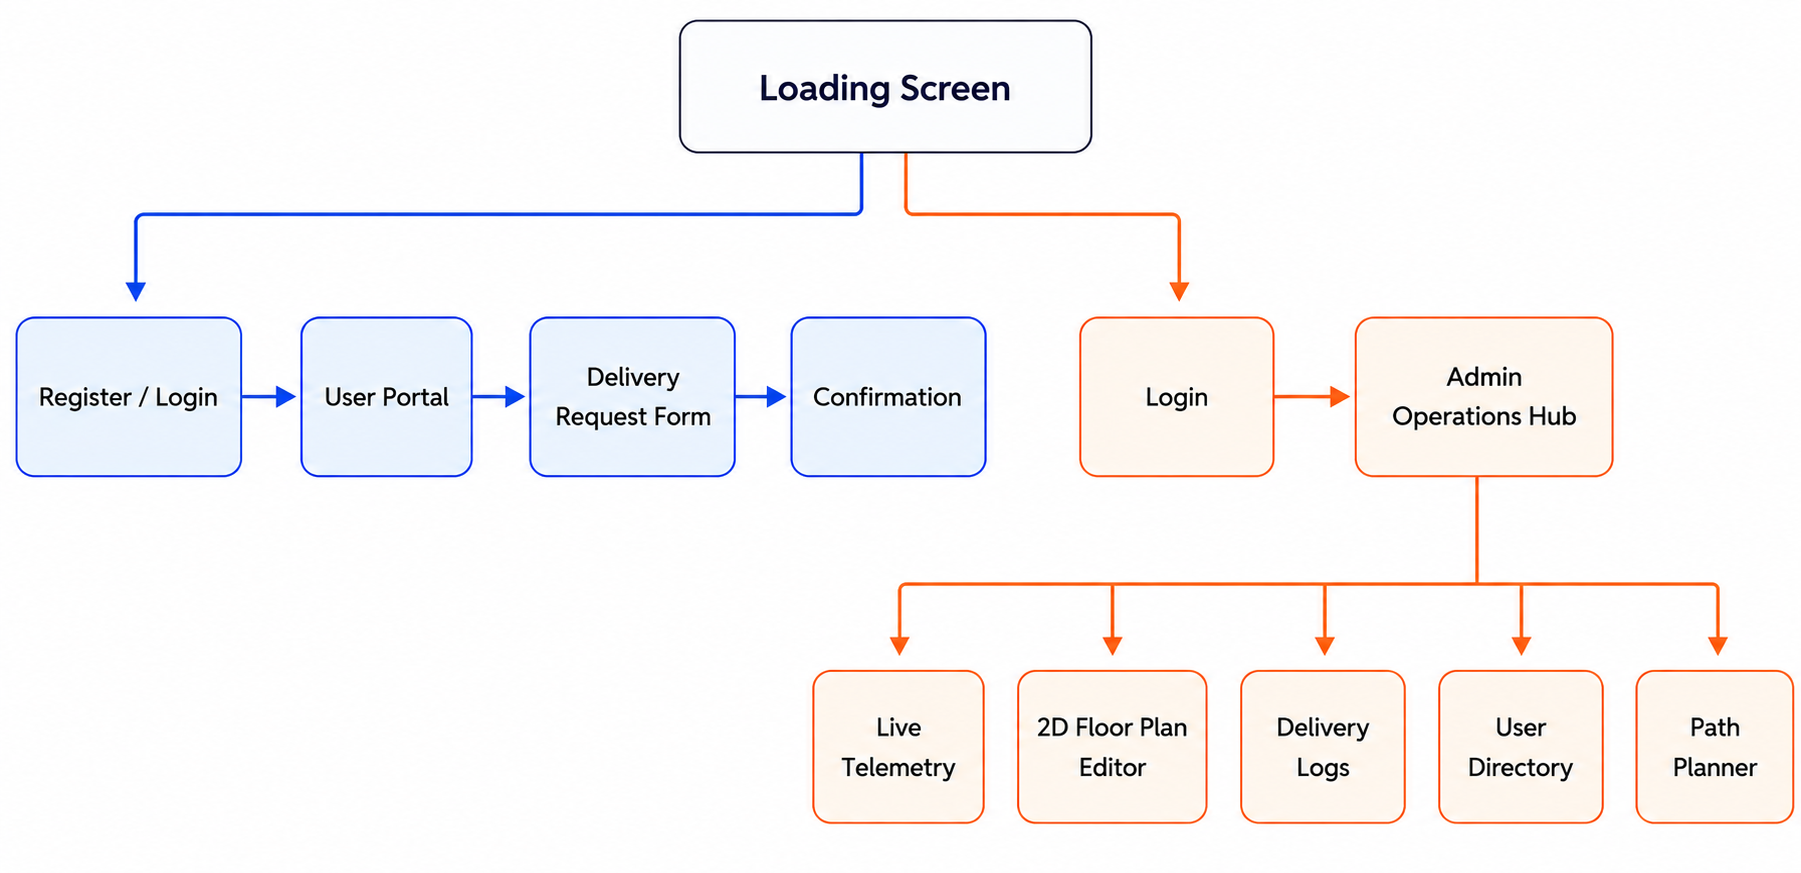
\includegraphics[width=0.9\textwidth]{app_screen_flow.png}
	\caption{Web screen flow, showing the separate user and administrator navigation paths}
	\label{fig:app_flow}
\end{figure}

\subsubsection{The Welcome Landing Screen}

With the headline \textit{``ParcelPath''} and the tagline \textit{``Autonomous indoor delivery, planned in real time''}, the application launches on a welcome landing screen that presents the platform. The user can access the login screen with just one \textbf{Get Started} action.


\subsubsection{Login and Registration}
The user is sent to either registration (complete name, email, and password) or login (registered email and password), both of which have password fields that are hidden, from the landing screen. New users can register straight from this flow, and the system ensures safe authentication by verifying email format and password strength before to submission.

\textbf{Routing based on roles.} Once the sign-in is successful, the backend identifies the user’s role and directs them to:

\begin{itemize}[noitemsep]
	\item \textbf{Users} are sent to the User’s Portal.
	\item \textbf{Administrators} are forwarded to the Admin Operations Hub.
\end{itemize}

\subsubsection{User Portal}
\label{sec:user_portal}
User Portal The main user interface is the User Portal, which shows a live status card and two necessary actions, requesting a new delivery and reviewing the delivery history record \textbf{Robot Status.} The status card represents the current state of the robot without revealing any ROS2-level information to the user. An idle robot is shown as \textit{free}, and an ongoing delivery is shown as \textit{busy} with its target room.

\textbf{Delivery Log.} The delivery history log lists each request together with its status and the date and time it was placed, so that users can track a delivery from submission through completion.

\textbf{Delivery Types.} The system supports two delivery types, distinguished by their pickup location:
\begin{itemize}[noitemsep]
	\item \textbf{Room to Room:} The robot travels from its home position to the specified pickup room to collect the parcel, then proceeds to the specified drop-off room, before finally returning to its home position.
	\item \textbf{Home to Room:} The robot's home position is itself the pickup location; the robot proceeds directly from home to the specified drop-off room and then returns.
\end{itemize}

\textbf{Requesting a New Delivery.} The Delivery Request form is centered on the same floor plan utilized to construct the Gazebo world. Rooms are represented as select blocks to enable delivery or pick-up/drop-off to be selected either from within the interactive map interface or by using its corresponding dropdown interface, to remove the need for the user to know coordinate system values. The selection live state displays a summary of rooms determined after selection. On confirmation, the backend resolves the selected rooms into their stored ROS navigation coordinates and begins the delivery process: if the robot is already free, the delivery is dispatched immediately; if the robot is busy with another delivery, the new request is queued and is automatically dispatched once the robot becomes free (or, in the case of a robot that is currently returning home, it may preempt the return trip, as described in Section~\ref{sec:fsm_design}).

\subsubsection{Admin Operations Hub (Command Center)}
\label{sec:admin_hub}

Administrators are routed to a separate Operations Hub rather than the delivery request screen. The hub presents an interactive grid layout of five independent modules, each represented by a custom line illustration that scales up slightly on hover. These modules are described below.

\textbf{Live Telemetry.} A dashboard showing the robot's real-time state. It streams the robot's $x, y$ coordinates (in metres), battery percentage, delivery queue length, and current order, and includes a live camera stream feed.

\textbf{2D Floor Plan Editor.} Allows administrators to edit and rename rooms in the building, and to update each room's coordinates so that a physical room maps to its exact pose on the map. Its design is presented in Section~\ref{sec:floor_plan_editor}.

\textbf{Path Planner.} Screen for configuring the path. It is based on an OpenStreetMap layout and offers drawing tools for workspace boundaries and circular/polygonal obstacles (static walls or furniture). It also provides solver buttons to execute A* search path calculations, cell decomposition and Particle Swarm Optimization (PSO) path smoothing. Its complete workflow is detailed in Section~3.4.3 (Phase 3: Web Platform Integration).

\textbf{Delivery Logs.} A history audit list of all deliveries with order times, status (pending, in-transit, completed) and dispatch profiles.

\textbf{User Directory.} An admin tool to list all registered users, and change their authorization roles (eg upgrade a user to Administrator) or flip their active status.

Table~\ref{tab:admin_modules} summarizes the functionality of these five modules.

\begin{table}[H]
	\centering
	\caption{Admin Operations Hub Modules}
	\label{tab:admin_modules}
	\begin{tabular}{|p{4cm}|p{10.5cm}|}
		\hline
		\textbf{Module} & \textbf{Functionality} \\
		\hline
		Live Telemetry & Streams robot position, battery percentage, queue length, current order, and live camera feed \\
		\hline
		2D Floor Plan Editor & Renames rooms and updates their navigation coordinates \\
		\hline
		Path Planner & Workspace/obstacle drawing and A*/cell-decomposition/PSO solver controls \\
		\hline
		Delivery Logs & Historical audit of all deliveries \\
		\hline
		User Directory & User role and account status management \\
		\hline
	\end{tabular}
\end{table}

\subsubsection{2D Floor Plan Editor Design}
\label{sec:floor_plan_editor}

The Floor Plan Editor is used to map each physical room to its coordinates in the robot’s navigation frame, so that the room choices provided in the delivery request form map to valid goal poses. From this screen, managers can rename rooms and adjust coordinates to keep room labels consistent with the actual facility. Each room entry is divided into two separate groups of fields deliberately: (i) \emph{visual layout} fields (bounding-box width/height and on-map position, edited as percentage sliders) that only control the room's on-screen drawing, and (ii) \emph{ROS navigation} fields ($x$, $y$, $\theta$) that control the robot's real goal pose. Table~\ref{tab:room_fields} illustrates this division, which enables the on-screen floor plan to be modified for visual clarity without risking accidental changes to the robot's calibrated delivery points.
\begin{table}[H]
	\centering
	\caption{Separation of Visual Layout and Navigation Fields in the Room Editor}
	\label{tab:room_fields}
	\begin{tabular}{|p{3.2cm}|p{4.5cm}|p{5.5cm}|}
		\hline
		\textbf{Field Group} & \textbf{Fields} & \textbf{Effect} \\
		\hline
		Visual Layout & label\_x, label\_y, region\_width, region\_height & Controls only how the room block is drawn on the floor plan (display-only) \\
		\hline
		ROS Navigation & x, y, theta & Defines the actual goal pose sent to Nav2 for that room \\
		\hline
	\end{tabular}
\end{table}

\subsubsection{Backend Server Development}

The backend server is implemented using the Python Flask framework and functions as the central coordination layer between the database, the path-planning algorithms, the web frontend and the ROS2 robotic stack. We use Flask routes to serve HTTP requests for map data, obstacle configuration, delivery management, robot telemetry, and user authentication and account management.

Table~\ref{tab:backend_files} summarizes the main backend files and their responsibilities.
\begin{longtable}{|p{0.8cm}|p{4.5cm}|p{8cm}|}
	\caption{Backend Files and Responsibilities}
	\label{tab:backend_files}\\
	
	\hline
	\textbf{Sr. No} & \textbf{File Name} & \textbf{Functionality Description} \\
	\hline
	\endfirsthead
	
	\hline
	\textbf{Sr. No} & \textbf{File Name} & \textbf{Functionality Description} \\
	\hline
	\endhead
	
	\hline
	\multicolumn{3}{|r|}{\textit{Continued on next page}} \\
	\hline
	\endfoot
	
	\hline
	\endlastfoot
	
	1 & server.py & Flask application entry point; defines REST API routes and coordinates all backend modules. \\
	\hline
	
	2 & models.py & Defines the database schema (User, Room, Delivery, Order, RobotState) using SQLAlchemy ORM. \\
	\hline
	
	3 & robot\_service.py & Implements the robot Finite State Machine (FSM) and manages ROS2 communication through rosbridge. \\
	\hline
	
	4 & astar\_modified.py & Implements the Improved A* path planning algorithm with obstacle inflation and path pruning. \\
	\hline
	
	5 & PSO\_path\_smothing.py / PSO\_implimentation.py & Implements Particle Swarm Optimization (PSO)-based path smoothing and cubic spline interpolation. \\
	\hline
	
\end{longtable}
The backend server does three main things:
\begin{itemize}[noitemsep]
	\item Accepts JSON data for map, obstacle, and delivery request
	\item Performs the selected path-planning pipeline and outputs computed trajectories
	\item Manages the robot's delivery Finite State Machine and sends navigation goals to ROS2
\end{itemize}

\subsubsection{Database Design}
\label{sec:db_design}

The system uses a relational SQLite database, through the SQLAlchemy ORM. Table~\ref{tab:db_schema} summarizes the core tables.

\begin{table}[H]
	\centering
	\caption{Core Database Tables}
	\label{tab:db_schema}
	\begin{tabular}{|p{2.5cm}|p{5cm}|p{6cm}|}
		\hline
		\textbf{Table} & \textbf{Key Fields} & \textbf{Purpose} \\
		\hline
		users & id, name, email, role & Stores login credentials and role-based access (admin/user) \\
		\hline
		rooms & id, name, x, y, theta, is\_robot\_home & Stores real-world coordinates of delivery locations \\
		\hline
		deliveries & id, sender\_id, recipient\_room\_id, status, scheduled\_at & Tracks the lifecycle of a delivery request from submission to completion \\
		\hline
		orders & id, type, pickup\_room, dropoff\_room, status & Low-level FSM task queue derived from deliveries \\
		\hline
		robot\_state & id, current\_status, x, y, battery\_level & Singleton table holding the robot's live FSM state, coordinates, and battery percentage \\
		\hline
	\end{tabular}
\end{table}

\subsubsection{Finite State Machine (FSM) Design}
\label{sec:fsm_design}

The delivery behaviour of the robot is controlled by a Finite State Machine implemented in the back-end and the current state is persisted to the robot state record described in Section~\ref{sec:db_design}. The FSM has four states: \textbf{free} (idle, parked at the home room), \textbf{en\_route\_to\_pickup} (moving to pick up a parcel for room-to-room deliveries), \textbf{en\_route\_to\_dropoff} (moving to the destination room), and \textbf{returning} (navigating back to home room after a completed delivery).

Transitions are triggered either by new delivery requests being written to the database or by success/failure callbacks from the ROS2 Nav2 action client. The complete state transition diagram is presented in Figure~\ref{fig:fsm}, and the transition logic is summarized in Table~\ref{tab:fsm_transitions}. The pickup and drop-off transitions are maintained on separate rows to correspond with the Room-to-Room and Home-to-Room delivery types described in Section~\ref{sec:user_portal}.

\begin{figure}[H]
	\centering
	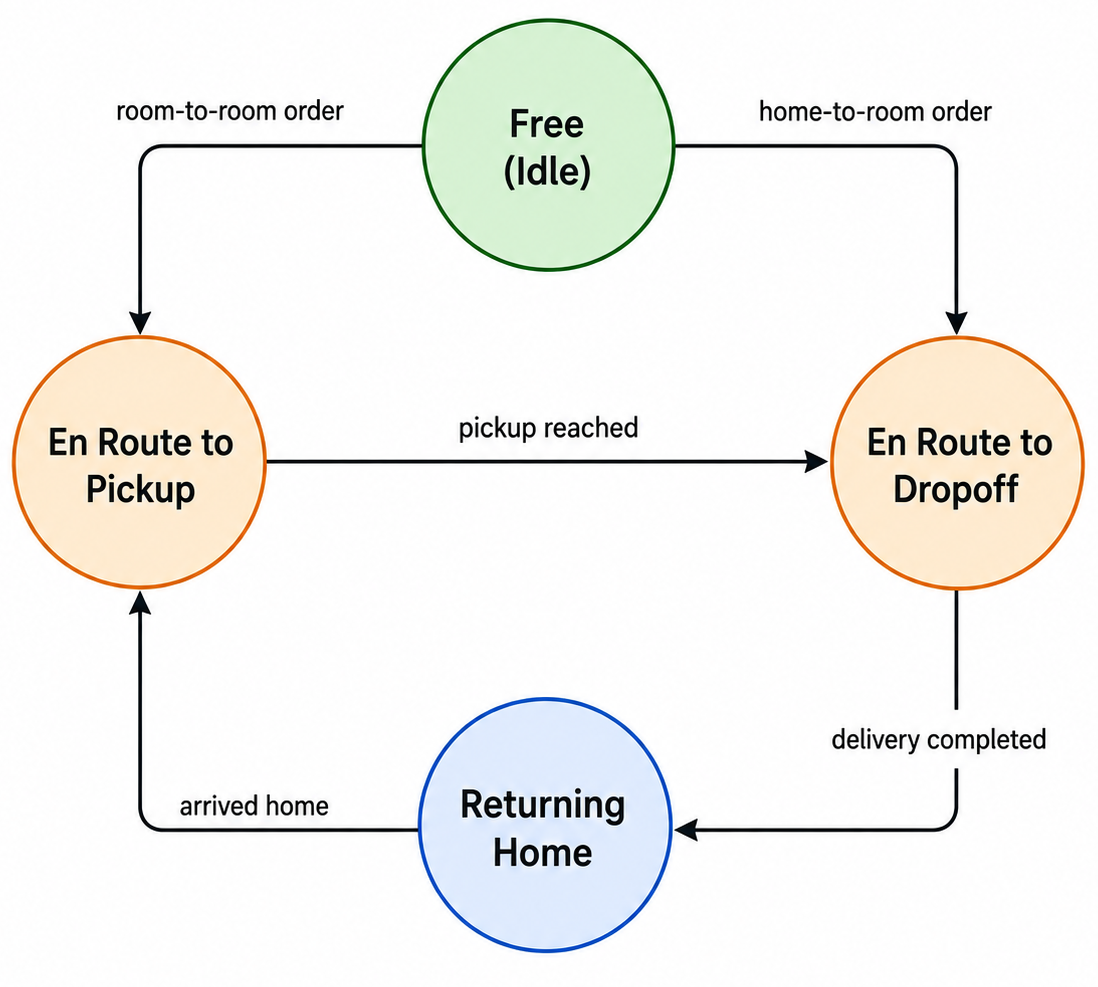
\includegraphics[width=0.6\textwidth]{fsm.png}
	\caption{Robot Delivery Finite State Machine (FSM)}
	\label{fig:fsm}
\end{figure}
\begin{longtable}{|p{3.2cm}|p{3.2cm}|p{7cm}|}
	\caption{FSM State Transitions}
	\label{tab:fsm_transitions}\\
	
	\hline
	\textbf{From State} & \textbf{To State} & \textbf{Trigger} \\
	\hline
	\endfirsthead
	
	\hline
	\textbf{From State} & \textbf{To State} & \textbf{Trigger} \\
	\hline
	\endhead
	
	\hline
	\multicolumn{3}{|r|}{\textit{Continued on next page}} \\
	\hline
	\endfoot
	
	\hline
	\endlastfoot
	
	free & en\_route\_to\_pickup & A new Room-to-Room order is dispatched; the robot must first travel to the pickup room. \\
	\hline
	
	free & en\_route\_to\_dropoff & A new Home-to-Room order is dispatched; the robot proceeds directly to the drop-off room. \\
	\hline
	
	en\_route\_to\_pickup & en\_route\_to\_dropoff & Robot reaches the pickup room (Nav2 goal succeeds). \\
	\hline
	
	en\_route\_to\_dropoff & returning & Robot reaches the destination room and the delivery is marked complete. \\
	\hline
	
	returning & free & Robot reaches the home room; the FSM checks for any queued orders. \\
	\hline
	
	returning & en\_route\_to\_pickup & A new Room-to-Room order arrives while returning. The current home-navigation goal is cancelled, and the robot is redirected to the pickup room. \\
	\hline
	
	returning & en\_route\_to\_dropoff & A new Home-to-Room order arrives while returning. The current home-navigation goal is cancelled, and the robot is redirected to the drop-off room. \\
	\hline
	
\end{longtable}
The preemption mechanism enables the robot to be redirected mid-return to a new delivery, without having to complete the trip home first, thus increasing the overall delivery throughput. It also implements the queuing behaviour exposed to the users on the User Portal (Section~\ref{sec:user_portal}): a request submitted while the robot is busy is simply stored as a pending order and automatically picked up by this same transition logic as soon as the robot becomes free.


\subsubsection{Backend-to-ROS2 Communication}

The Flask backend communicates with the ROS2 stack asynchronously via WebSockets, so there is no need to run ROS2 nodes inside the Flask process. A rosbridge\_websocket server (rosbridge\_suite) is run on port 9090 and the backend connects to it as a client via the roslibpy library. The communication path is shown in Figure~\ref{fig:ros_bridge}.

\begin{figure}[H]
	\centering
	
\includegraphics[width=0.8\textwidth]{ros2 bridge architecture.png}
	\caption{Backend-to-ROS2 Communication Architecture via rosbridge}
	\label{fig:ros_bridge}
\end{figure}

Table~\ref{tab:ros2_topics} summarizes the key ROS2 interfaces used in this communication. The Interface column indicates whether the channel is a Topic or an Action, and the Data Type column gives the specific ROS2 message or action type carried on that channel.

\begin{table}[H]
	\centering
	\caption{ROS2 Topics, Services, and Actions Used}
	\label{tab:ros2_topics}
	\begin{tabular}{|p{3cm}|p{2.3cm}|p{8.7cm}|}
		\hline
		\textbf{Channel} & \textbf{Interface} & \textbf{Role} \\
		\hline
		/navigate\_to\_pose & Action & Receives navigation goals from the backend FSM \\
		\hline
		/amcl\_pose & Topic & Publishes robot pose; read by backend to update telemetry \\
		\hline
		/plan & Topic & Publishes the active global trajectory; read by backend for display \\
		\hline
		/cmd\_vel & Topic & Velocity commands from the Nav2/MPPI controller to the simulated robot \\
		\hline
		/scan & Topic & Simulated LiDAR data for localization and costmaps \\
		\hline
		/camera/image\_raw & Topic & Camera stream, relayed to the web interface's Live Telemetry module \\
		\hline
		/battery\_state (simulated) & Topic & Simulated battery telemetry, relayed to the robot state record and displayed as a percentage in the Live Telemetry module and User Portal status card \\
		\hline
	\end{tabular}
\end{table}



\section{Phase 5: ROS2 \& Gazebo Setup}
\label{sec:phase5_ros2_gazebo}

In this section, the virtual machine, the operating system, the ROS2 distribution, the Gazebo simulator and the TurtleBot3 Waffle robot model are presented. This project did not need any physical hardware, as it is entirely simulation based where the entire navigation stack has been developed and tested in this virtual environment.


\subsection{Virtual Machine and Ubuntu Setup}
\label{subsec:vm_ubuntu_setup}

ROS2 and Gazebo are Linux native, so a Linux virtual machine was built on top of the host operating system using \textbf{Oracle VirtualBox}. The virtual machine was set up with at least two processing cores, 4 GB RAM and network connectivity to download packages. The ROS2 Humble distribution is officially supported on the platform Ubuntu 22.04 LTS \textbf(Jammy Jellyfish), which was installed as the guest operating system. System packages were updated after the installation to be compatible with software that would be added later.

\subsection{Gazebo 11 Classic Installation} \label{subsec:gazebo_install} \textbf{Gazebo Classic 11} was selected as the physics simulation platform, because it is the version officially coupled with ROS2 Humble via the ROS-Gazebo bridge packages. 
The Gazebo simulator and its ROS2 integration packages were installed together and the installation was verified by opening Gazebo directly to verify that it opened correctly. \subsection{TurtleBot3 Packages Installation} \label{subsec:turtlebot3_install} The simulated robot platform used was the \textbf{TurtleBot3 Waffle} robot model. All the TurtleBot3 packages were installed using the ROS2 package manager and the robot model was configured to Waffle by setting the corresponding environment variable, which was also saved permanently so it persists in the following terminal sessions.
 \subsection{ROS2 Workspace Creation} \label{subsec:ros2_workspace} All the custom packages and nodes developed for this project were maintained in a dedicated ROS2 workspace. The workspace had some custom elements such as the MPC controller node, the trajectory publisher and the custom world files. The workspace was built with ROS2’s build tool and its setup file was sourced (and added to the shell startup file, after the ROS2 Humble source line) so that all custom packages are available in addition to the basic ROS2 installation in every new terminal session.
 \subsection{World Creation} \label{subsec:gazebo_world_creation} A custom Gazebo world was developed to mimic a realistic indoor environment for testing the proposed autonomous delivery system. The environment is composed of 4 rooms linked by a central hallway, offering a mix of open spaces and narrow passages to challenge the robot’s navigation in various scenarios. Each room was furnished with different Gazebo models to emulate an indoor facility in the real world (desks, chairs, sofas, cabinets, tables, waiting areas, and other indoor fixtures). One room was dedicated as a \textbf{robot room}, which was the robot's starting place before it performed delivery tasks.Variation in furniture placement and room layouts creates a realistic environment with static obstacles as well as narrow passages to navigate through. To test the ability of the robot to work in dynamic environments, a model of a walking person was added to the simulation as a moving obstacle. This dynamic obstacle with unpredictable motion is used to test the navigation system for real-time detection, avoidance and path replanning. To launch the whole simulation environment with the TurtleBot3 Waffle robot, a dedicated ROS~2 launch file was employed. The TurtleBot3 Waffle robot provides a realistic testbed for autonomous indoor navigation and delivery experiments.

\subsubsection*{Room Coordinate Mapping}

Within each room, a known position was to be chosen as a pickup or drop-off point in the ParcelPath web interface (Phase 4) in the simulated environment. To locate these positions, a reference point was manually defined at the desired delivery location in each room of the Gazebo world. The corresponding $(x,y)$ coordinates of the selected point were then obtained directly from the \textit{Property} panel of Gazebo, which displays the pose of the selected object in the world reference frame. This procedure was performed for each room, producing a fixed set of coordinates which were then registered in the 2D Floor Plan Editor as valid navigation goals.

\begin{figure}[H]
	\centering
	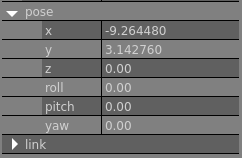
\includegraphics[width=0.4\textwidth]{coor.png}
	\caption{Gazebo Property panel displaying the world coordinates $(x,y)$ }
	\label{fig:gazebo_coordinates}
\end{figure}

The robot's home position, called the \textbf{Robo Room}, was intentionally placed near the world origin at approximately $(0,0)$ to facilitate initialization and navigation. Table~\ref{tab:room_coordinates} lists the recorded coordinates for all rooms in the simulated environment.

\begin{table}[H]
	\centering
	\caption{Registered Room Coordinates}
	\label{tab:room_coordinates}
	\begin{tabular}{|c|p{3cm}|p{3cm}|p{3cm}|}
		\hline
		\textbf{ID} & \textbf{Name} & \textbf{X Coordinate} & \textbf{Y Coordinate} \\
		\hline
		1 & Room 1 & -14.6662 & 2.28722 \\
		\hline
		2 & Room 2 & -9.26448 & 3.14276 \\
		\hline
		3 & Room 3 & -14.9200 & -1.62217 \\
		\hline
		4 & Room 4 & -9.00083 & -2.43645 \\
		\hline
		5 & Robo Room & 0.0000 & 0.0000 \\
		\hline
	\end{tabular}
\end{table}

These recorded coordinates are used to map the actual rooms in the Gazebo environment to the corresponding delivery locations in the ParcelPath web interface .

\subsection{Environment Configuration Summary}
\label{subsec:gazebo_config_summary}

Table~\ref{tab:gazebo_configuration_p5} summarizes the complete simulation environment configuration.

\begin{table}[H]
	\centering
	\caption{Gazebo Simulation Environment Configuration}
	\label{tab:gazebo_configuration_p5}
	\begin{tabular}{|p{3.5cm}|p{10cm}|}
		\hline
		\textbf{Component} & \textbf{Description} \\
		\hline
		Virtualization & Oracle VirtualBox \\
		\hline
		Operating System & Ubuntu 22.04 LTS (Jammy Jellyfish) \\
		\hline
		ROS Distribution & ROS2 Humble Hawksbill \\
		\hline
		Simulation Platform & Gazebo 11 Classic \\
		\hline
		Robot Model & TurtleBot3 Waffle \\
		\hline
		Environment Design & Four rooms with one Robo room connected by a hallway, with a dynamic walking-person obstacle \\
		\hline
		Visualization & RViz2 for real-time monitoring \\
		\hline
		Physics Engine & ODE (Open Dynamics Engine) \\
		\hline
	\end{tabular}
\end{table}


\subsection{Navigation Reliability Assessment in Dynamic Environments}

The time of execution of both A* and dynamic planning algorithms in order to compare their efficiencies in terms of algorithms to the varied map complexities.

\begin{itemize}[noitemsep]
	\item Path replanning capability
	\item Obstacle avoidance consistency
	\item Robot stability under dynamic disturbances
	\item Controller response to environmental changes
\end{itemize}


The test establishes that the navigation structure works well in the real world. Table~\ref{tab:performance_metrics} lists the performance metrics used in the course of the navigation analysis, including quality of path, smoothness, tracking accuracy, computational efficiency, and reliability, which allows performing a full assessment of the system.
% Table 3.1
\begin{table}[H]
	\centering
	\caption{Performance Evaluation Metrics Used for Navigation Analysis}
	\label{tab:performance_metrics}
	\begin{tabular}{|p{3.5cm}|p{3.5cm}|p{5.5cm}|}
		\hline
		\textbf{Evaluation Category} & \textbf{Metric} & \textbf{Description} \\
		\hline
		Path Quality & Path Length & Total distance traveled by robot \\
		\hline
		Path Smoothness & Curvature Continuity & Measures directional consistency \\
		\hline
		Tracking Accuracy & Tracking Error & Deviation from reference trajectory \\
		\hline
		Computational Efficiency & Algorithm Execution Time & Time required for path planning and optimization \\
		\hline
		Reliability & Obstacle Avoidance Success Rate & Ability to avoid static and dynamic obstacles \\
		\hline
	\end{tabular}
\end{table}

% ============================================================
% UPDATED REPLACEMENT BLOCK for chapter3.tex (v3)
% Covers: Phase 2 (Web Interface) through System Integration and Testing
% Paste this in place of the corresponding existing block.
% Uses the same \subsection / \subsubsection formatting already
% defined in main.tex — no formatting commands changed.
%
% CHANGES IN THIS VERSION:
%   - Admin Operations Hub modules (previously an A/B/C/D/E
%     description list) are now individual bold lead-in paragraphs
%     ("Live Telemetry.", "2D Floor Plan Editor.", etc.), matching
%     the style already used in the User Portal subsection — no
%     more lettered list.
%   - Removed \texttt{CustomPainter} styling from the prose; the
%     Admin Hub intro now describes the hover illustrations without
%     naming the specific Flutter widget class.
%   - "Admin Operations Hub Modules and Source Files" table is now
%     a 2-column table (Module, Functionality): the Source File
%     column and the A./B./C. letter prefixes have been removed.
%   - FSM State Transitions table: rows that previously combined
%     two destination states in one cell (e.g. "en_route_to_pickup
%     / en_route_to_dropoff") are now split into separate rows, one
%     transition per row, with the Room-to-Room vs Home-to-Room
%     distinction stated explicitly in the trigger column.
%   - ROS2 Topics table: fixed an inconsistent message-type string
%     (the /amcl_pose row was missing "/msg/", unlike every other
%     row) and relabelled the columns (Interface / Data Type) so
%     the Type and Message/Action columns no longer read as
%     duplicates of each other.
% ============================================================

\section{Phase 6: MPPI Navigation}
\label{sec:phase7_mppi}

While the MPC controller (Phase 3) tracks the smoothed global path under nominal conditions, it relies on a fixed cost formulation and struggles to react quickly to unexpected, close-range disturbances such as a moving obstacle suddenly entering the robot's path. To address this, \textbf{Model Predictive Path Integral (MPPI) control} was introduced as a local planner, working alongside the global planning pipeline (Phases 1--2) to detect and avoid dynamic obstacles particularly a person walking through the robot's path in real time.

\subsection{What is MPPI}
\label{subsec:mppi_overview}

Model Predictive Path Integral (MPPI) is a sampling-based model predictive control method. Unlike traditional MPC, which solves a constrained optimization problem analytically or through gradient-based solvers, MPPI works by randomly generating many possible future control sequences rollouts, simulating the outcome of each one using the robot's motion model, scoring each rollout with a cost function, and then combining them into a single weighted-average control command.

This sampling-based approach has several practical advantages for local, reactive navigation:

\begin{itemize}[noitemsep]
	\item It does not require the cost function or motion model to be smooth or differentiable, so arbitrarily complex costs (e.g. sharp obstacle penalties) can be used directly.
	\item It naturally handles nonlinear dynamics and non-convex obstacle constraints, which are difficult for gradient-based MPC to optimize reliably.
	\item It can be updated at high frequency, making it well suited for reacting to sudden, dynamic obstacles such as a walking person crossing the robot's path.
\end{itemize}

For these reasons, MPPI was integrated as the \textbf{local planner}, responsible for short-horizon, reactive obstacle avoidance, while the global planner (A* with PSO smoothing) remains responsible for long-horizon route planning across the full environment.

\subsection{Local Planning with MPPI}
\label{subsec:mppi_local_planning}

At every control cycle, the MPPI local planner performs the following steps:

\begin{enumerate}[noitemsep]
	\item \textbf{Sample} a large number ($K$) of candidate control sequences, each consisting of a short sequence of linear and angular velocity commands, by perturbing a nominal control sequence with random noise.
	\item \textbf{Simulate (rollout)} each candidate sequence forward through the robot's kinematic model over a short prediction horizon, producing $K$ candidate future trajectories.
	\item \textbf{Evaluate} each candidate trajectory using a cost function that penalizes deviation from the local reference path, proximity to obstacles (including the dynamic walking-person obstacle), and excessive control effort.
	\item \textbf{Weight} each candidate trajectory using a soft-min (exponential) weighting based on its cost 
	\item \textbf{Combine} all weighted candidate control sequences into a single optimal control sequence.
	\item \textbf{Apply} only the first control command of this combined sequence to the robot, then repeat the entire process at the next control cycle (receding horizon, similar to Phase 3).
\end{enumerate}

Because MPPI operates over a short horizon and reacts directly to real-time sensor data (LiDAR-detected obstacles), it complements the global planner by handling situations the global plan could not anticipate, such as a person walking into the corridor after the global path was already computed.

\subsection{Mathematical Formulation}
\label{subsec:mppi_math}

Given a nominal control sequence $U = (u_0, u_1, \dots, u_{N-1})$, MPPI generates $K$ perturbed control sequences:

\begin{equation}
	u_k^{(i)} = u_k + \epsilon_k^{(i)}, \qquad i = 1, \dots, K
	\label{eq:mppi_perturbation}
\end{equation}

where $\epsilon_k^{(i)} \sim \mathcal{N}(0, \Sigma)$ is Gaussian noise sampled independently for each rollout $i$ and each time step $k$, with covariance $\Sigma$.

Each rollout $i$ is assigned a cost $S^{(i)}$, accumulated over the horizon:

\begin{equation}
	S^{(i)} = \sum_{k=0}^{N-1} c(x_k^{(i)}, u_k^{(i)}) + c_{terminal}(x_N^{(i)})
	\label{eq:mppi_cost}
\end{equation}

where $c(x_k, u_k)$ is the running cost (tracking error, obstacle penalty, control effort) and $c_{terminal}$ penalizes the final predicted state.

The optimal control update is computed as a cost-weighted average over all rollouts:

\begin{equation}
	u_k^{*} = u_k + \frac{\sum_{i=1}^{K} \exp\left(-\frac{1}{\lambda} S^{(i)}\right) \epsilon_k^{(i)}}{\sum_{i=1}^{K} \exp\left(-\frac{1}{\lambda} S^{(i)}\right)}
	\label{eq:mppi_update}
\end{equation}

where $\lambda$ is a temperature parameter which can be used to trade-off the preference of the lowest cost rollouts and the higher cost rollouts: a smaller $\lambda$ gives more weight to the lowest cost rollouts, while a larger $\lambda$ gives a more averaged result.
\subsection{Parameters}
\label{subsec:mppi_parameters}
Table~\ref{tab:mppi_parameters} summarizes the MPPI local planner configuration used in this project.

\begin{longtable}{|p{5cm}|p{2.5cm}|p{6cm}|}
	\caption{MPPI Local Planner Parameters}
	\label{tab:mppi_parameters} \\
	
	\hline
	\textbf{Parameter} & \textbf{Symbol} & \textbf{Value} \\
	\hline
	\endfirsthead
	
	\hline
	\textbf{Parameter} & \textbf{Symbol} & \textbf{Value} \\
	\hline
	\endhead
	
	\hline
	\multicolumn{3}{r}{\textit{Continued on next page}} \\
	\hline
	\endfoot
	
	\hline
	\endlastfoot
	
	Number of Samples (Rollouts) &
	$K$ &
	1000 \\
	\hline
	
	Prediction Horizon &
	$N$ &
	30 steps \\
	\hline
	
	Sampling Time &
	$\Delta t$ &
	0.05 seconds \\
	\hline
	
	Temperature Parameter &
	$\lambda$ &
	1.0 \\
	\hline
	
	Control Noise Standard Deviation (linear velocity) &
	$\sigma_v$ &
	0.2 m/s \\
	\hline
	
	Control Noise Standard Deviation (angular velocity) &
	$\sigma_\omega$ &
	0.4 rad/s \\
	\hline
	
	Linear Velocity Limits &
	$v$ &
	$v \in [0,0.26]$ m/s \\
	\hline
	
	Angular Velocity Limits &
	$\omega$ &
	$\omega \in [-1.9,1.9]$ rad/s \\
	\hline
	
	Obstacle Cost Weight &
	-- &
	50.0 \\
	\hline
	
	Path Tracking Cost Weight &
	-- &
	10.0 \\
	\hline
	
	Minimum Safe Obstacle Distance &
	-- &
	0.35 m \\
	\hline
	
\end{longtable}
1000 sample paths provide the controller with sufficient options to choose the most secure path without exceeding the maximum processing time per step. The low value of temperature ($\lambda=1.0$) makes the robot commit strongly to the single best path it finds, rather than blend it with riskier options -- so it reacts quickly and decisively when the person gets close. Finally, the obstacle avoidance weight (50.0) is set much higher than the path following weight (10.0) so the robot is happy to deviate from the original path to avoid a collision rather than strictly following its route.

\subsection{Integration with the Global Planner}
\label{subsec:mppi_integration}

MPPI operates as a local planning layer on top of the global path produced in Phases 1 and 2, forming a two-tier navigation architecture:

\begin{itemize}[noitemsep]
	\item The \textbf{global planner} (Improved A* with PSO smoothing) computes a long-horizon, obstacle-free path across the entire known map, based on the static occupancy grid.
	\item The \textbf{local planner} (MPPI) continuously tracks a short rolling section of this global path, while reacting in real time to LiDAR sensor data that may reveal dynamic obstacles  most notably the \textbf{walking person} present in the Gazebo simulation world (Phase 5) that are not represented in the original static map.
\end{itemize}

At each control cycle, the local reference segment for MPPI is extracted from the nearest upcoming portion of the global path. Under normal conditions, with no dynamic obstacles nearby, MPPI closely tracks this reference segment, producing motion very similar to the underlying MPC tracking behavior (Phase 3). However, when the walking-person obstacle moves into or near the robot's planned path, the obstacle cost term in the MPPI cost function (Equation~\ref{eq:mppi_cost}) sharply penalizes any rollout that passes too close to the obstacle's detected position. Since MPPI evaluates a large number of randomly sampled trajectories at every cycle, it naturally identifies alternative rollouts that steer around the obstacle while still making progress toward the local goal, and the weighted combination of these low-cost rollouts produces a smooth avoidance maneuver.

Once the dynamic obstacle is out of the way of the robot, the obstacle cost term is no longer dominant and the path tracking cost term pulls the robot back to the original global path. This multi-layered design takes advantage of the benefits of both planners: the global planner ensures that the robot has always an efficient and complete path to the goal, while the local MPPI planner ensures safe, reactive behavior in the presence of unpredictable, real-time disturbances, like a person walking in the corridor that the global planner cannot anticipate in advance.



\section{Phase 7: Rviz setting }

\subsection{RViz Visualization Configuration}

For visualization of the custom navigation stack outputs during simulation, RViz2 was configured with dedicated Path displays for the raw global planner output and the optimized trajectory for control. Figure~\ref{fig:rviz_settings}
shows the corresponding display settings.

The raw global path generated by the Improved A* planner is subscribed from the \textit{/plan} topic and visualized in green Lines style (RGB: 25, 255, 0).
The pruned and PSO-smoothed trajectory from the \textit{/plan\_smoothed} topic is plotted separately with blue Lines style (RGB: 0, 170, 255). For both displays the buffer length is 1, thus only the most recently published path is displayed at any time, instead of the accumulated older paths from previous planning cycles.
This configuration allows for real time visual comparison of the raw A* output and the PSO-smoothed path within the same scene, allowing for direct observation of the effect of the pruning and smoothing stages on the quality of the path.
The Model Predictive Controller subscribes to the smoothed path on \textit{/plan\_smoothed} and uses it as the reference trajectory to generate the velocity commands that drive the robot’s motion.

\begin{figure}[h]
	\centering
	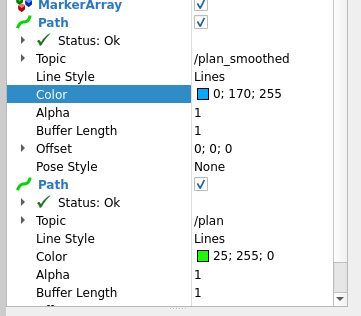
\includegraphics[width=0.5\textwidth]{setting.png}
	\caption{RViz configuration showing the raw A* global path
		and the PSO-smoothed path used as	the reference trajectory for the MPC controller.}
	\label{fig:rviz_settings}
\end{figure}

\section{Design of the Project Hardware}

The current project is fully a simulation project and does not need any physical hardware design and development. The autonomous navigation system, such as the modeling of the robot, the process of sensor integration, the creation of the environment, the execution of the path planning and the tracking of the trajectory are all implemented and tested in Gazebo simulation environment with ROS2 with Jazzy. The TurtleBot3 Waffle robot example is the virtual hardware platform and all specifications, sensors, and motion dynamic specifications are defined by the parameters in the simulation process, which ensures the whole system development and testing process are done in a fully virtual environment without the necessity of having any physical hardware components.

\section{Details of Final Working Prototype}
\label{sec:final_prototype}

The final working prototype integrates all six development phases described in
the preceding sections into a single, end-to-end simulated delivery pipeline. The
complete system is brought online through a fixed startup sequence executed across
multiple terminals, after which the robot is able to autonomously accept, plan, and
execute delivery tasks issued from the web interface.
The prototype requires five independent processes to be launched in sequence, each
in its own terminal, before the system becomes fully operational:
\begin{enumerate}
	\item \textbf{Gazebo Simulation:} The custom indoor world,
	together with the TurtleBot3 Waffle robot model, is launched using the
	project's ROS 2 launch file. This initializes the physics simulation,
	the robot's sensors (LiDAR and RGB camera), and the dynamic walking-person
	obstacle.
	
	\item \textbf{RViz Visualization:} RViz2 is launched to provide real-time
	visualization of the occupancy map, the robot's localized pose, the planned
	global path, and the local MPPI-adjusted trajectory during navigation.
	
	\item \textbf{Rosbridge WebSocket Server:} The rosbridge server is started
	on port 9090 to expose the ROS 2 communication layer to the Flask backend
	by running ros2 launch rosbridge\_server rosbridge\_websocket\_launch.xml.
	This bridge is what allows the backend to publish navigation goals and
	subscribe to telemetry, pose, and battery topics over a standard WebSocket
	connection rather than requiring a native ROS 2 client.
	
	\item \textbf{Camera Streaming Server:} The web\_video\_server
	package is launched to relay the robot's RGB camera feed as an
	HTTP-accessible video stream by running ros2 run web\_video\_server
	web\_video\_server. This stream is used directly by the Live Telemetry module of the Admin Operations Hub.
	
	\item \textbf{Backend and Frontend Servers:} Finally, the Flask backend server (server.py) and the Flutter frontend (ParcelPath) are started, completing the software stack and making the web application available to the user.
\end{enumerate}
\subsection*{End-to-End Delivery Workflow}

With the prototype fully launched, a complete delivery is executed as follows:

\begin{enumerate}
	\item \textbf{Authentication.} The user logs in through the ParcelPath
	landing screen and is routed, based on their role, to either the User
	Portal or the Admin Operations Hub
	
	\item \textbf{Task Assignment.} A user creates a delivery request simply by selecting their drop-off and/or pickup room from the interactive map/room selection menu and confirms the request. The mapped/selected rooms are resolved to their programmed navigation co-ordinates, and these co-ordinates are communicated back to the backend.
	
	\item \textbf{Dispatch and Queuing.} The backend's Finite State Machine
 checks the robot's current status. If the
	robot is the delivery is dispatched immediately; otherwise,
	the request is stored as a pending order and automatically dispatched once
	the robot becomes available.
	
	\item \textbf{Path Planning.} Upon dispatching, the backend call the whole
	planning pipeline, which consists of: An Improved A* planning a collision-free trajectory on the
	grid Path pruning that get rid of unnecessary points and PSO based smoothing algorithm that generates a
	kinematically feasible trajectory in an ongoing curve.
	\item \textbf{Trajectory Tracking.} The smoothed trajectory is published
	to ROS 2 and subscribed to by the MPC controller node in RViz/Gazebo, which computes velocity commands to
	track the path while respecting the robot's kinematic and actuator
	constraints.
	
	\item \textbf{Dynamic Obstacle Avoidance.} While executing the planned
	trajectory, the MPPI local planner continuously monitors LiDAR data for unexpected obstacles, most notably the
	walking-person model in the simulation, and reactively adjusts the robot's
	short-horizon motion to avoid collisions before resuming the original path.
	
	\item \textbf{Live Monitoring.} As it’s running the robot’s position, battery life, and delivery state is broadcast back to the web application interface. Admins will also want to watch the progress of the delivery using Live Telemetry to see where the robot is in real-time, together with its live camera Feed sent over Web video service.
	\item \textbf{Completion and Return.} When the delivery is completed and the FSM reaches the drop-off room, it becomes marked as completed in the database, and the FSM changes its current state from route to dropoff to returning back towards Robo Room. If when the robot reaches home, there are no other deliveries in the delivery pipeline, then the FSM changes from returning to free and the robot stays at home doing nothing, till a new delivery request comes. But if in case of any other delivery request when the robot was on its way home to reach the Free state, then the currently pursuing home-navigation goal is cancelled, and the robot will start heading towards the pickup or the dropoff location of the new order, without completing the return journey, therefore reducing delay of new delivery.
\end{enumerate}

\begin{figure}[h]
	\centering
	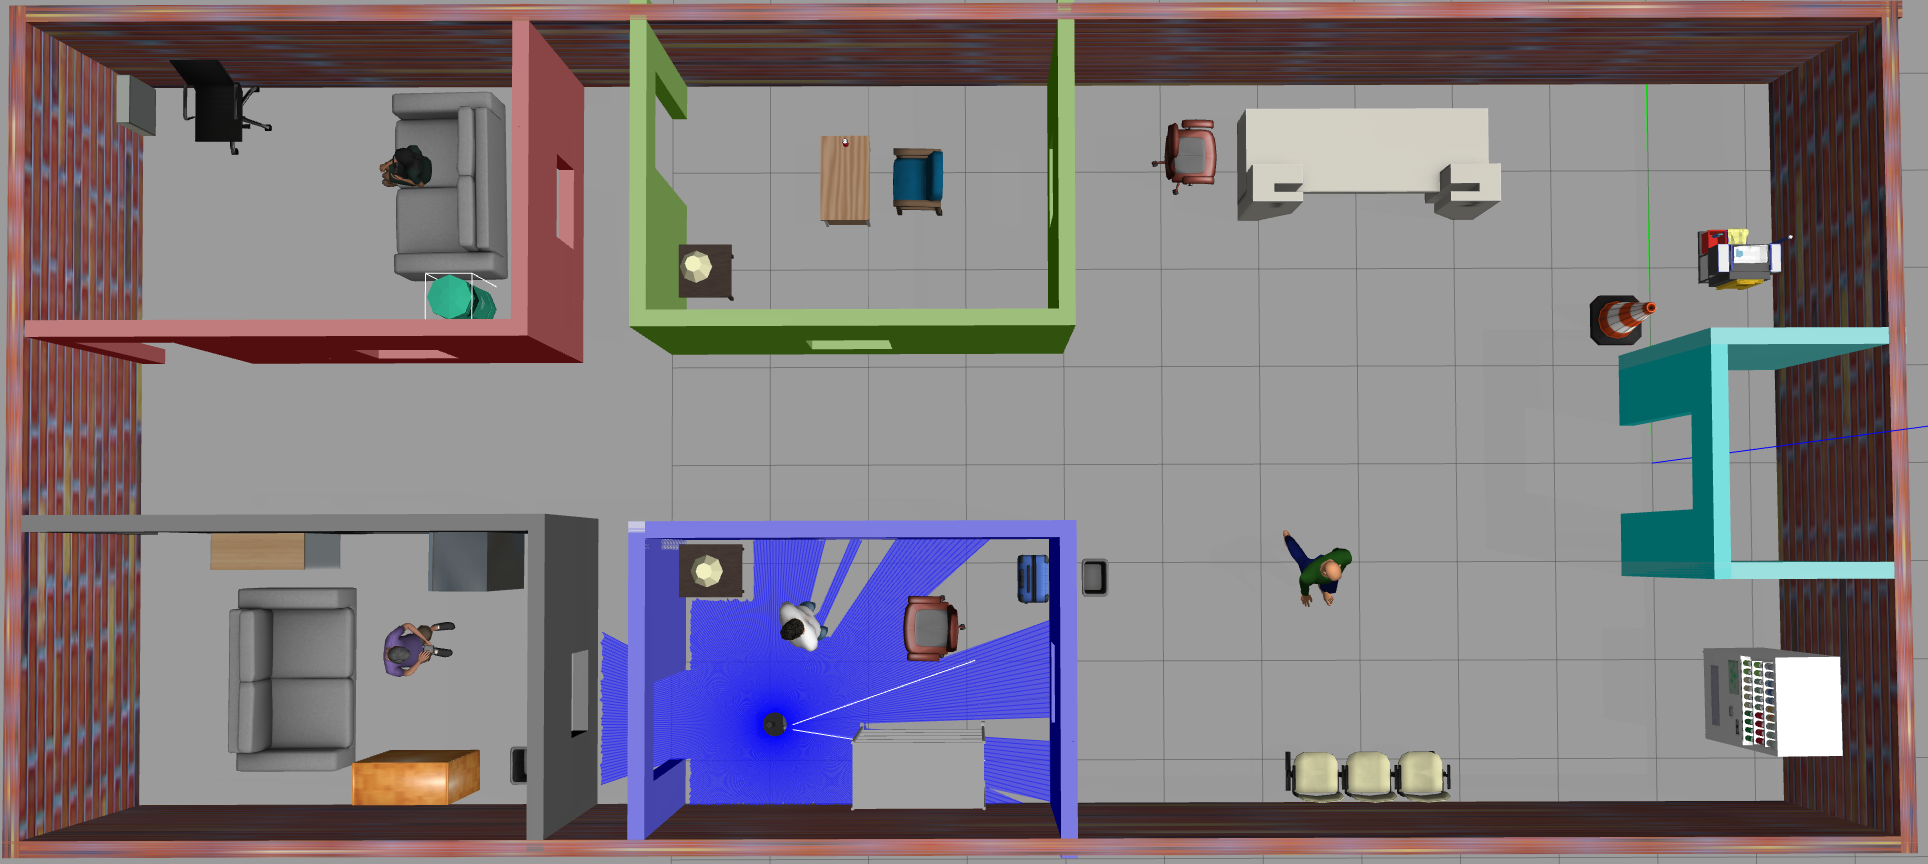
\includegraphics[width=0.75\textwidth]{gazebo_marking_robot_at_delivery_point}
	\caption{TurtleBot3 Waffle robot completing delivery task at
		the destination.}
	\label{fig:delivery_complete}
\end{figure}

This complete workflow,spanning task assignment, global path planning,
smoothing, MPC-based tracking, MPPI-based dynamic obstacle avoidance,
real-time telemetry, and FSM-driven dispatch (including mid-return
preemption for queued orders)  demonstrates that the proposed system
successfully integrates all six development phases into a functioning,
simulation-based autonomous parcel delivery prototype.
\section{Chapter Summary}
\label{sec:chapter_summary}

This chapter presented the design and implementation of the autonomous parcel
delivery system, developed through six phases: global path planning, path
optimization, controller design, web and backend development, ROS2/Gazebo
simulation setup, and MPPI-based dynamic obstacle avoidance.The Improved A* algorithm generated collision-free global paths, which were
pruned and smoothed using Particle Swarm Optimization to produce short,
feasible trajectories. A Model Predictive Controller tracked these paths whilerespecting the robot's motion constraints, and an MPPI local planner was addedto reactively avoid dynamic obstacles such as a moving person.
A web platform, ParcelPath, was built with a Flutter frontend and Flask
backend to let users request deliveries and let admins monitor the robot via
live telemetry and camera feed.A Finite State Machine handled the delivery dispatch and the queuing and preemption upon return, communicating with ROS2 via rosbridge. The entire system was tested in a custom Gazebo world with TurtleBot3 with reliable path planning, smooth trajectory tracking, and effective obstacle avoidance, all fully simulated without any physical hardware.